
%(BEGIN_QUESTION)
% Copyright 2007, Tony R. Kuphaldt, released under the Creative Commons Attribution License (v 1.0)
% This means you may do almost anything with this work of mine, so long as you give me proper credit

Examine this P\&ID:
 
$$\includegraphics[width=15.5cm]{i01660x01.eps}$$

The ``feed conveyor'' introduces granular material into the hopper, where the pile's height is measured by a guided-wave radar level transmitter.  The ``demand conveyor'' draws material from the bottom of the hopper as needed to supply another process.
 
What will happen to the level inside the hopper over time if one conveyor moves more material than the other?

\vskip 10pt

Would you characterize this process as inherently {\it self-regulating} or inherently {\it integrating}?

\underbar{file i01660}
%(END_QUESTION)





%(BEGIN_ANSWER)

The level inside the hopper will drift either up or down (depending on which conveyor moves more material) at a rate determined by the differential material flow ($Q_{in}$ $-$ $Q_{out}$).  This makes it an {\it integrating} process.

\vskip 10pt

Integrating processes are characterized by the capacity to experience persistent mass and/or energy imbalances, where the out-flow of mass and/or energy does not naturally reach equilibrium the in-flow over time.  Self-regulating processes, by contrast, naturally equalize their mass and energy balances as the process variable changes.

%(END_ANSWER)





%(BEGIN_NOTES)

Integrating processes are characterized by mass and/or energy imbalances, where the out-flow of mass and/or energy does not naturally reach equilibrium the in-flow over time.

%INDEX% Control, process characteristics: self-regulating versus integrating

%(END_NOTES)


